\documentclass[journal=jpcbfk]{achemso}

\usepackage[version=3]{mhchem}
\usepackage[T1]{fontenc}
\newcommand*\mycommand[1]{\texttt{\emph{#1}}}
\newcommand{\todo}[1]{\textcolor{red}{#1}}

\usepackage{rotating}
\usepackage{upgreek}				
\usepackage{xcolor}
\usepackage{booktabs}
\usepackage{multirow}
\usepackage{lmodern}
\usepackage{microtype}
\usepackage{xr}
\externaldocument{manuscriptPGPE}
\usepackage{soul} % for highlights with \hl{} 

\author{Pavel Buslaev}
\affiliation{University of Jyv{\"a}skyl{\"a}}

\author{Fernando Favela-Rosales}
\affiliation[Tecnol\'{o}gico Nacional de M\'{e}xico]{Departamento de Investigaci\'{o}n, Tecnol\'{o}gico Nacional de M\'{e}xico, Campus Zacatecas Occidente, M\'{e}xico}

\author{Patrick Fuchs}
\affiliation{Paris, France}

\author{Matti Javanainen}
\affiliation[Czech Academy of Sciences]{Institute of Organic Chemistry and Biochemistry of the 
Czech Academy of Sciences, Flemingovo n\'{a}m. 542/2, CZ-16610 Prague 6, Czech Republic}

\author{Jesper J. Madsen}
\affiliation[University of Chicago]{Department of Chemistry, The University of Chicago, Chicago, Illinois, United States of America}
\alsoaffiliation[University of South Florida]{Department of Global Health, College of Public Health, University of South Florida, Tampa, Florida, United States of America}

\author{Josef Melcr}
\affiliation[Czech Academy of Sciences]{Institute of Organic Chemistry and Biochemistry of the 
Czech Academy of Sciences, Flemingovo n\'{a}m. 542/2, CZ-16610 Prague 6, Czech Republic}
\alsoaffiliation{Groningen Biomolecular Sciences and Biotechnology Institute 
and The Zernike Institute for Advanced Materials, 
University of Groningen, 9747 AG Groningen, The Netherlands}


\author{Markus S. Miettinen}
% \affiliation[Max Planck Institute of Colloids and Interfaces]{Department of Theory and Bio-Systems, Max Planck Institute of Colloids and Interfaces, 14424 Potsdam, Germany}
\affiliation{Department of Theory and Bio-Systems, Max Planck Institute of Colloids and Interfaces, 14424 Potsdam, Germany}

\author{O. H. Samuli Ollila}
\email{samuli.ollila@helsinki.fi}
\affiliation{Institute of Biotechnology, University of Helsinki}

\author{Chris G. Papadopoulos}
\affiliation[]{I2BC - University Paris Sud}


\author{Antonio Pe{\'o}n}
\affiliation[]{Spain}

\author{Thomas J. Piggot}
\affiliation[University of Southampton]{Chemistry, University of Southampton, Highfield, Southampton SO17 1BJ, United Kingdom}

\author{Pierre Poulain}
\affiliation{Paris, France}

%\author{O. H. Samuli Ollila}
%\email{samuli.ollila@helsinki.fi}
%%\homepage[]{Your web page}
%\affiliation{Institute of Organic Chemistry and Biochemistry,
%Academy of Sciences of the Czech Republic, 
%Prague 6, Czech Republic}
%\affiliation{Institute of Biotechnology, University of Helsinki}


\SectionNumbersOn

\renewcommand{\thetable}{S\arabic{table}}%
\renewcommand{\thefigure}{S\arabic{figure}}%
\renewcommand{\thesection}{S\arabic{section}}%
\renewcommand{\thepage}{S\arabic{page}}%

\title{ Supporting Information:\\ NMRlipids IV: Headgroup \& glycerol backbone structures, and cation binding in bilayers with PE and PG lipids }

\begin{document}

\newpage
%\tableofcontents

\section{Simulated systems}

\subsection{CHARMM36}

\noindent {\it POPE} \todo{Simulation details by M. Javanainen}.

\noindent {\it POPE with additional NaCl} \todo{Simulation details by A. Peon.}

\noindent {\it POPG} \todo{Simulation details by Ollila}.

\noindent {\it POPG with additional NaCl} \todo{Simulation details by A. Peon.}

\noindent {\it POPC:POPE mixtures} Data is available at \cite{POPCcharmm300K,POPC1POPE1charmm36}.
300 K with v-rescale (tau=0.1 ps),
1 bar with PR semiisotropic (tau=4 ps, compressibility=4.5e-5 bar$^{-1}$),
PME order 4 and space 0.12,
rcoulomb and rvdw 1.0,
128 lipids per leaflet,
no ion \todo{Full simulation details by Fuchs et al.}

\noindent {\it POPC:POPG mixture with additional calcium} \todo{Simulation details by J. Madsen.}

\noindent {\it POPC:POPG mixture with additional NaCl} \todo{Simulation details by A. Peon.}

\subsection{CHARMM36ua}

\noindent {\it POPE} Data is available at \cite{charmm36uaPOPEfiles}. \todo{Simulation details by  T. Piggot.}

%\subsection{MacRog}

%\subsection{Lipid17}

\subsection{Slipids}
\noindent {\it POPE} Data is available at \cite{slipidsPOPEfiles}. \todo{Simulation details by  T. Piggot.}

\noindent {\it POPE with additional NaCl} \todo{Simulation details by A. Peon.}

\noindent {\it DPPE} Data is available at \cite{slipidsDPPEfiles}. \todo{Simulation details by F. Favela.}

\noindent {\it POPG} Data is available at \cite{slipidsPOPGfiles}. \todo{Simulation details by F. Favela.}

\noindent {\it POPG with additional NaCl} \todo{Simulation details by A. Peon.}

\noindent {\it DPPG} Data in 298~K is available at \cite{slipidsDPPGfilesT298K} and in 314~K at \cite{slipidsDPPGfiles}.  \todo{Simulation details by F. Favela.}

\noindent {\it POPC:POPG mixture with additional NaCl} \todo{Simulation details by A. Peon.}

\subsection{Berger}

\noindent {\it POPE} Data is available at \cite{bergerPOPEfiles,berger2POPEfiles}. \todo{Simulation details by  T. Piggot.}

\noindent {\it DOPE} Data is available at \cite{bergerDOPEfiles,berger2DOPEfiles}. \todo{Simulation details by  T. Piggot.}

\noindent {\it POPC:POPE, POPC:DOPE and DOPC:DOPE mixtures} Data is available at \cite{POPCberger300K,POPC1POPE1berger}. 
300 K with v-rescale (tau=0.1 ps),
1 bar with PR semiisotropic (tau=4 ps, compressibility=4.5e-5 bar$^{-1}$),
PME order 4 and space 0.12,
rcoulomb and rvdw 1.0,
128 lipids per leaflet,
no ion \todo{Simulation details by Fuchs et al.}

\subsection{GROMOS 43A1-S3}

\noindent {\it POPE} Data is available at \cite{gromos43a1s3POPEfiles}. \todo{Simulation details by  T. Piggot.}

\subsection{OPLS-UA}

\noindent {\it POPE} Data is available at \cite{OPLSuaPOPEfiles}. \todo{Simulation details by  T. Piggot.}

\noindent {\it POPE with vdW interaction in H} Data is available at \cite{OPLSuaWvdWPOPEfiles}. \todo{Simulation details by  T. Piggot.}

\subsection{GROMOS-CKP and GROMOS-CKPM}

\noindent {\it POPE} Data is available at \cite{gromosCKPpope}. \todo{Simulation details by  T. Piggot.}

\noindent {\it DOPE} Data is available at \cite{gromosCKPdope}. \todo{Simulation details by  T. Piggot.}

\noindent {\it DPPE} Data is available at \cite{gromosCKPdppe}. \todo{Simulation details by  T. Piggot.}

\clearpage
\section{R-PDLF and SDROSS experiments}

\begin{figure}[]
%  \centering
  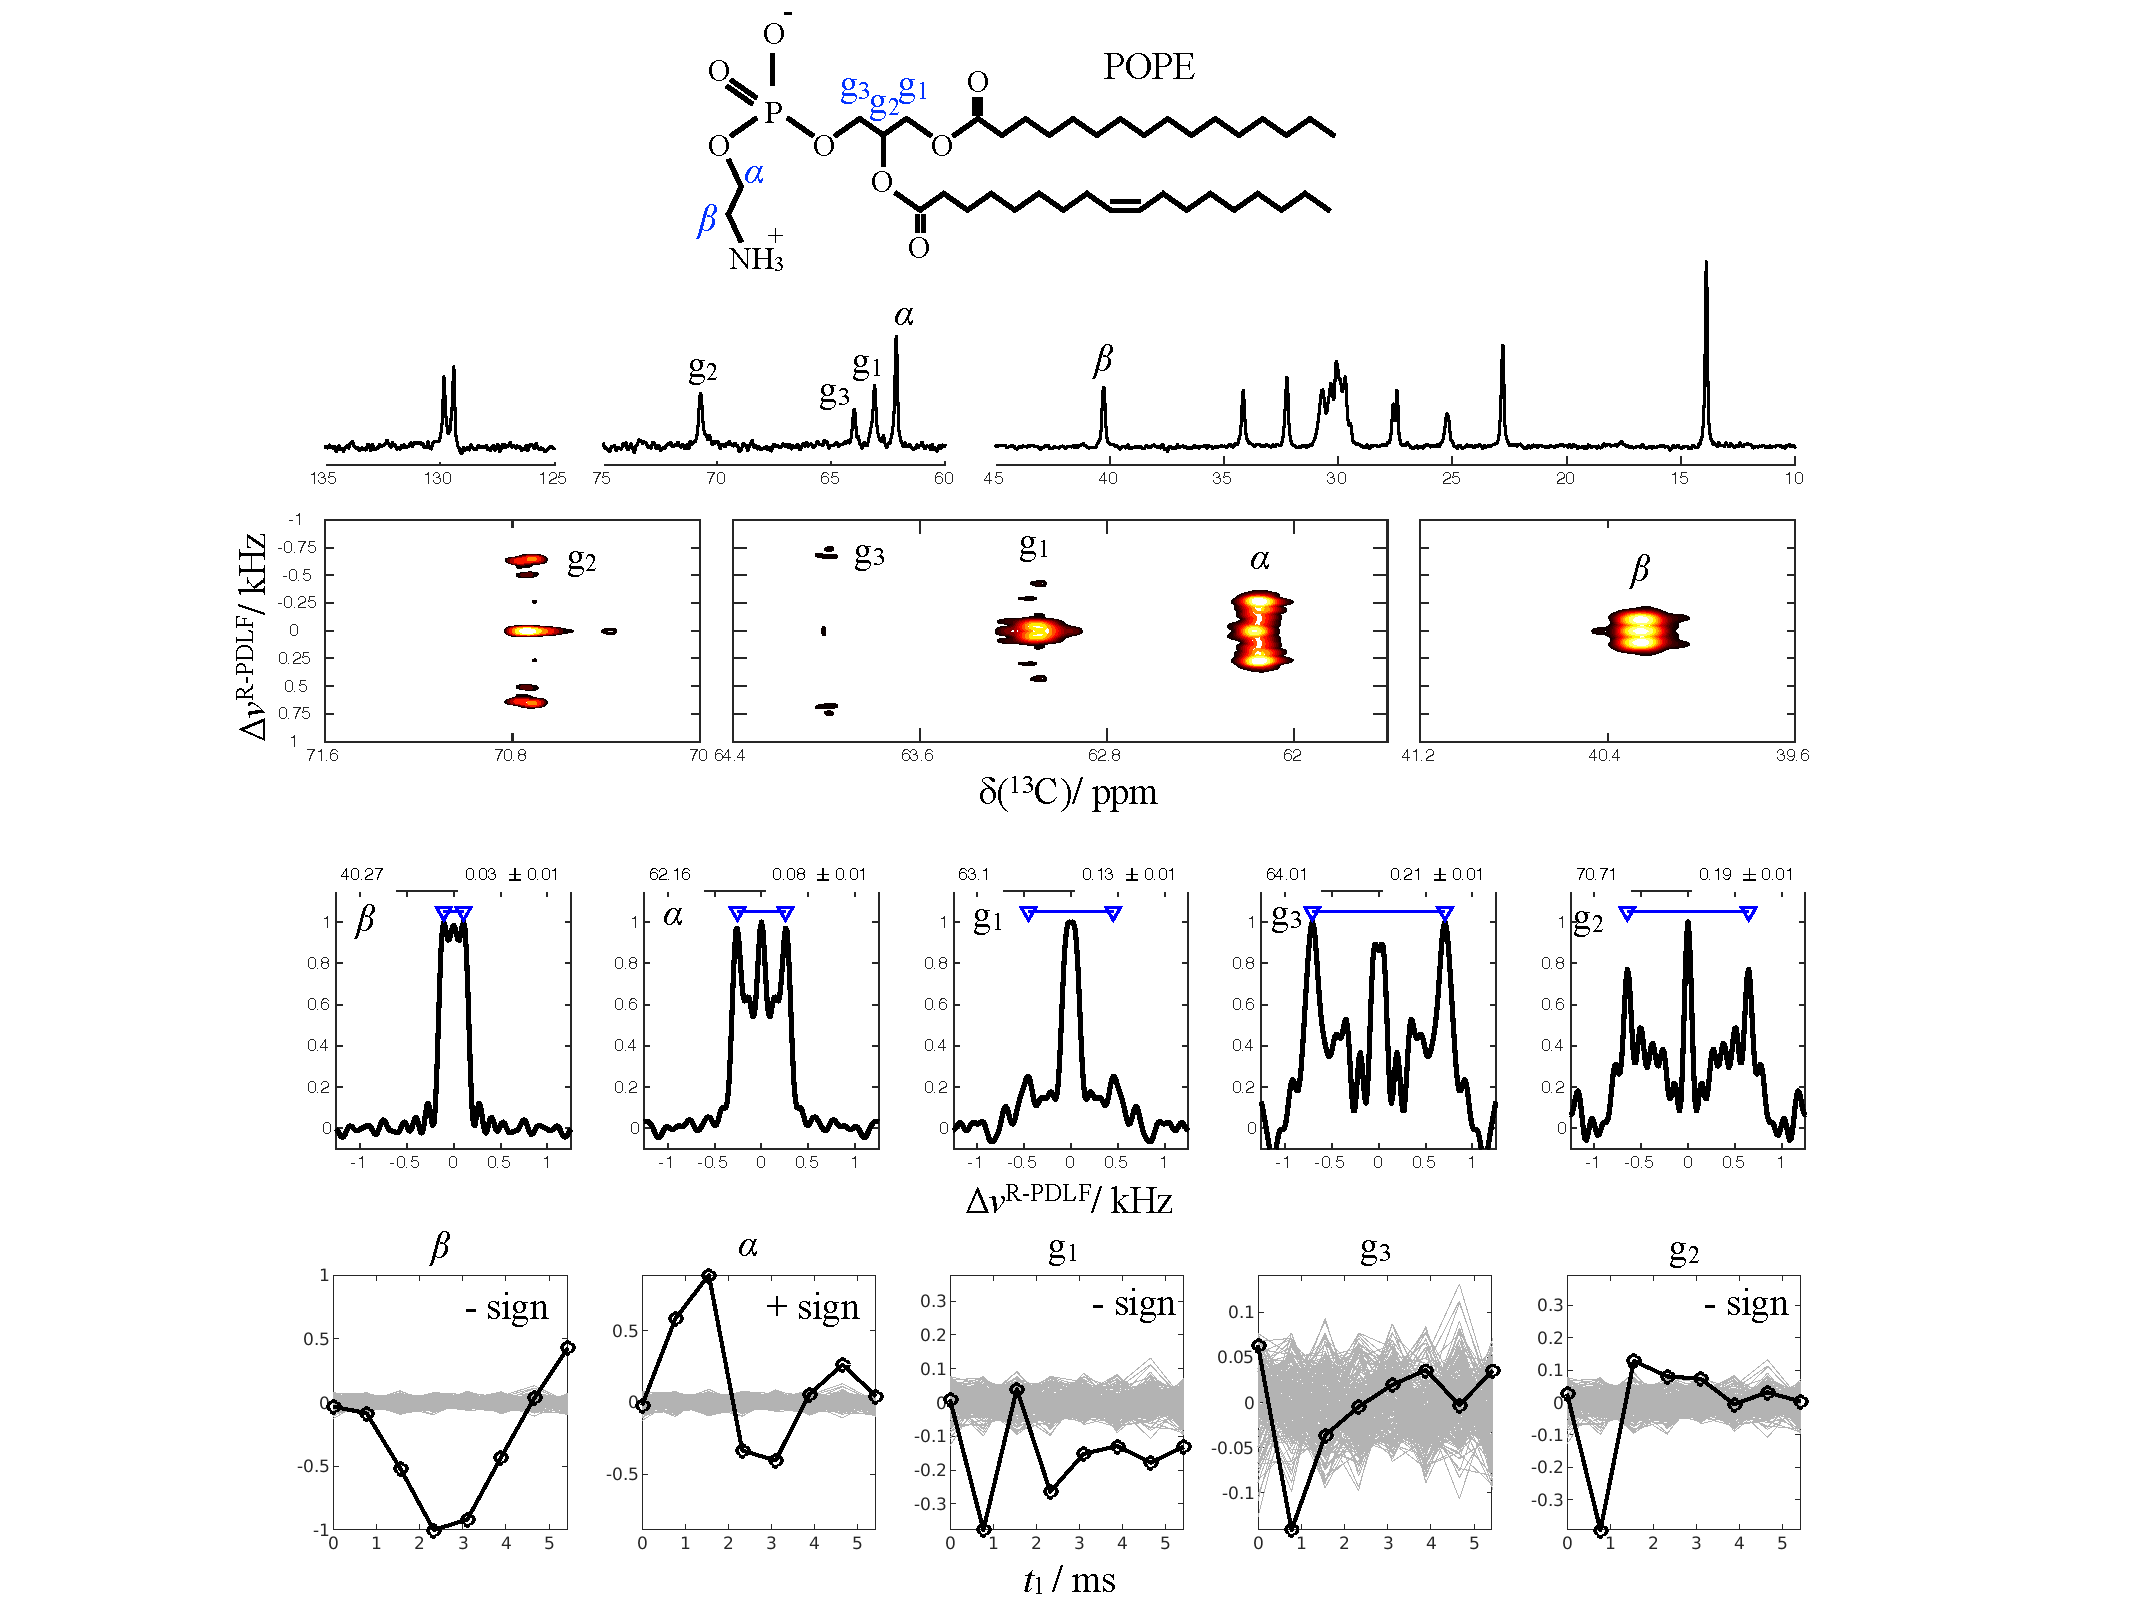
\includegraphics[width=0.8\textwidth]{../Figs/POPEexperiment.pdf}
  \caption{\label{POPEspectra}
    (A) Chemical structure of POPE with the labeling of headgroup and glycerol backbone carbons.
    (B) INEPT spectra from POPE sample with the headgroup and glycerol backbone peaks labeled.
    (C) 2D R-PDLF spectra
    (D) Dipolar sliced from the  2D R-PDLF spectra with the resulting order parameters on top of figures.
    (E) Experimetal S-DROSS curves giving signs of the order parameters.
  }
  \todo{A, B etc. labels to be put in the figure.}
\end{figure}

\begin{figure}[]
%  \centering
  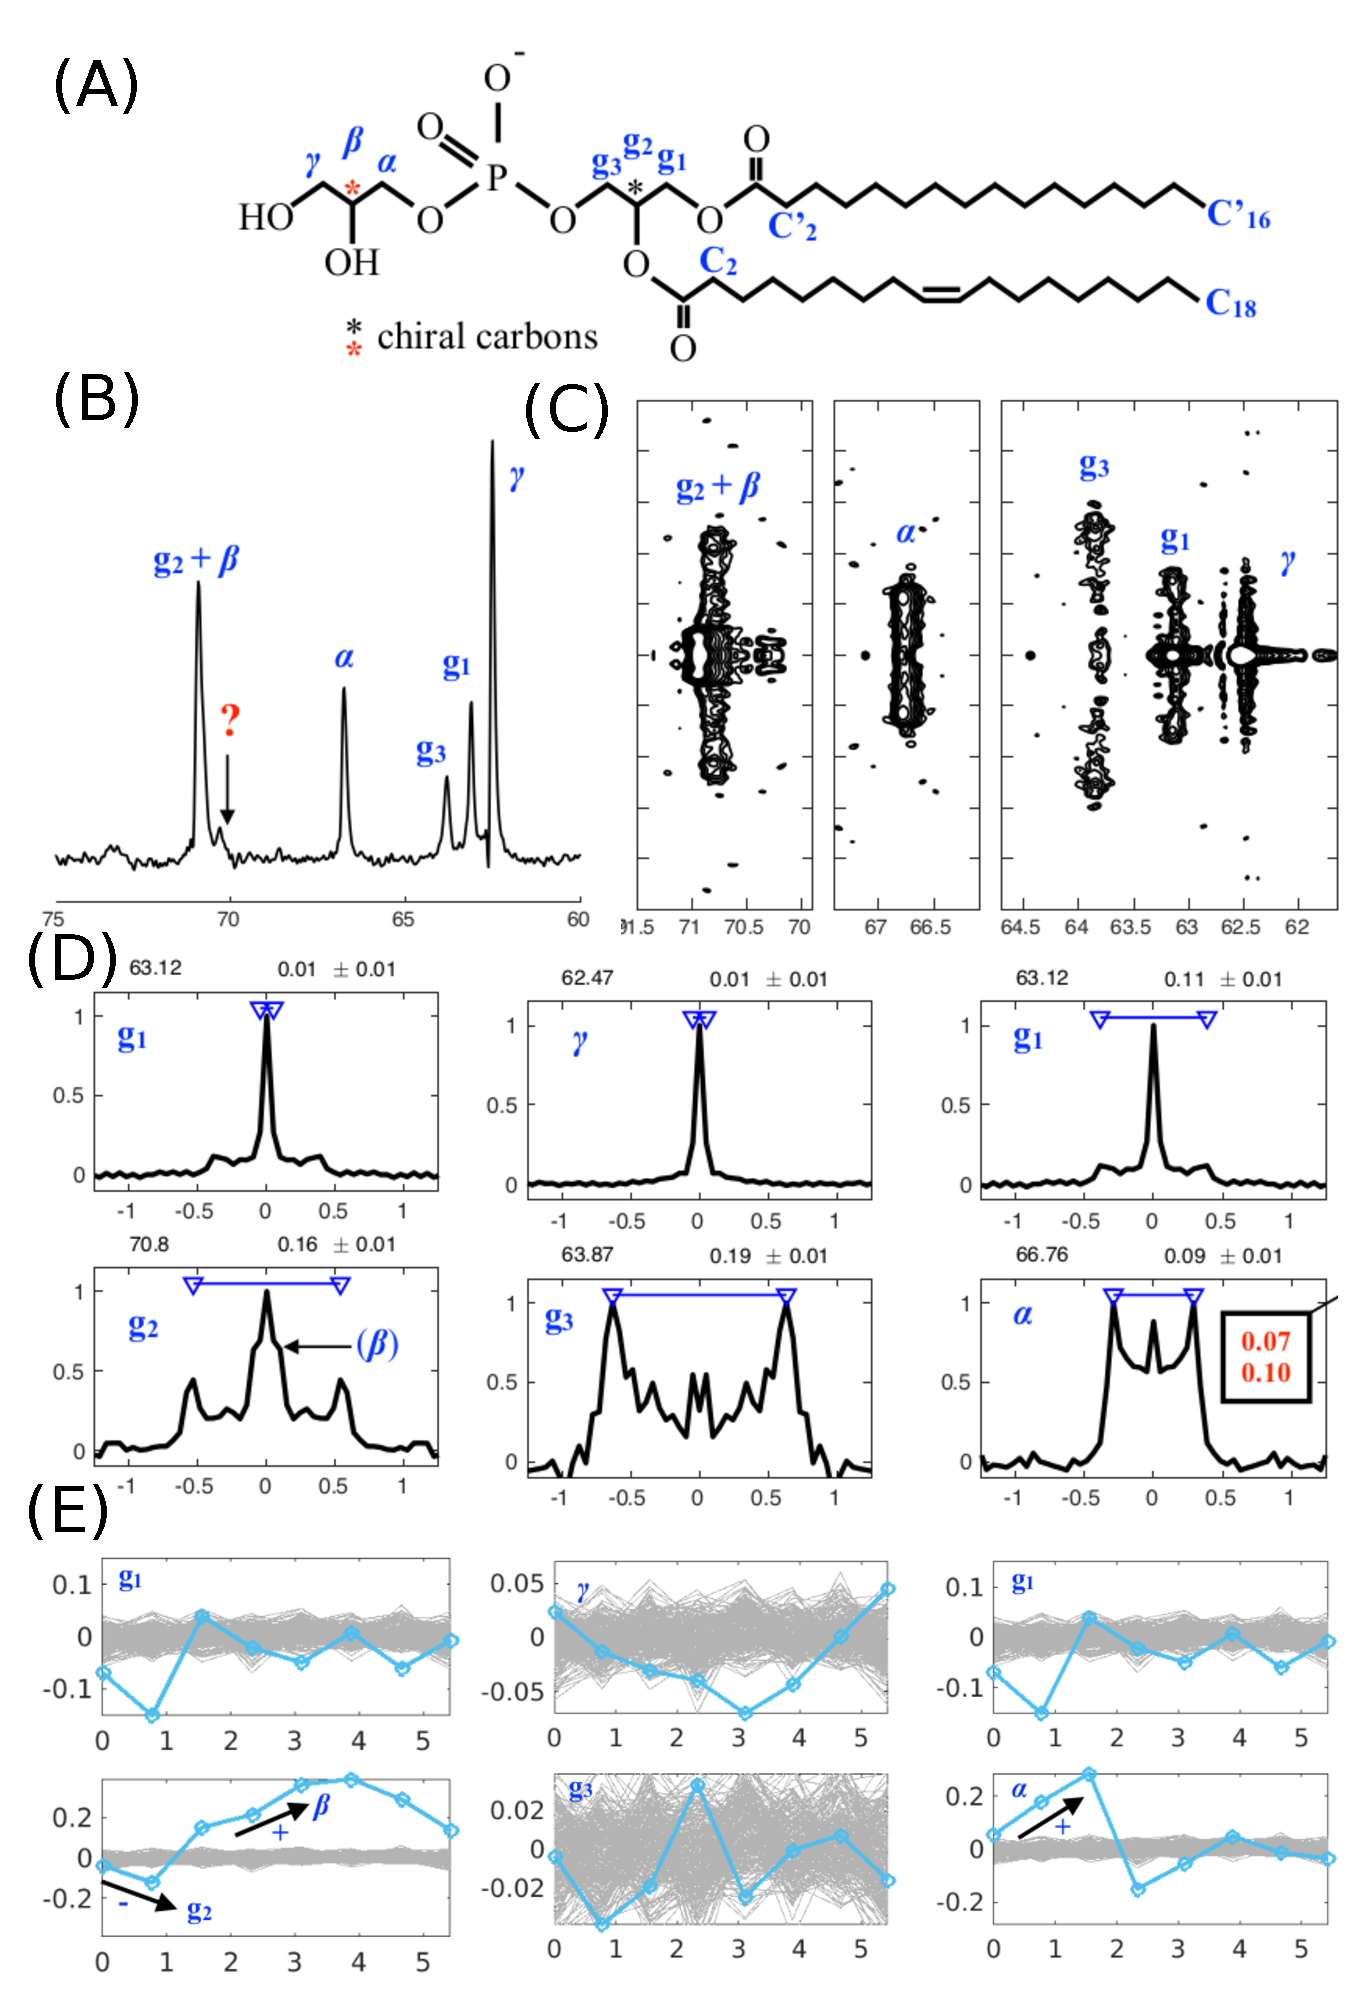
\includegraphics[width=0.8\textwidth]{../Figs/PGexpRPDLF.eps}
  \caption{\label{POPGspectra}
    (A) Chemical structure of POPG with the labeling of headgroup and glycerol backbone carbons.
    (B) INEPT spectra from POPG sample with the headgroup and glycerol backbone peaks labeled.
    (C) 2D R-PDLF spectra
    (D) Dipolar sliced from the  2D R-PDLF spectra with the resulting order parameters on top of figures.
    (E) Experimetal S-DROSS curves giving signs of the order parameters.
  }
\end{figure}

\begin{figure}[]
%  \centering
  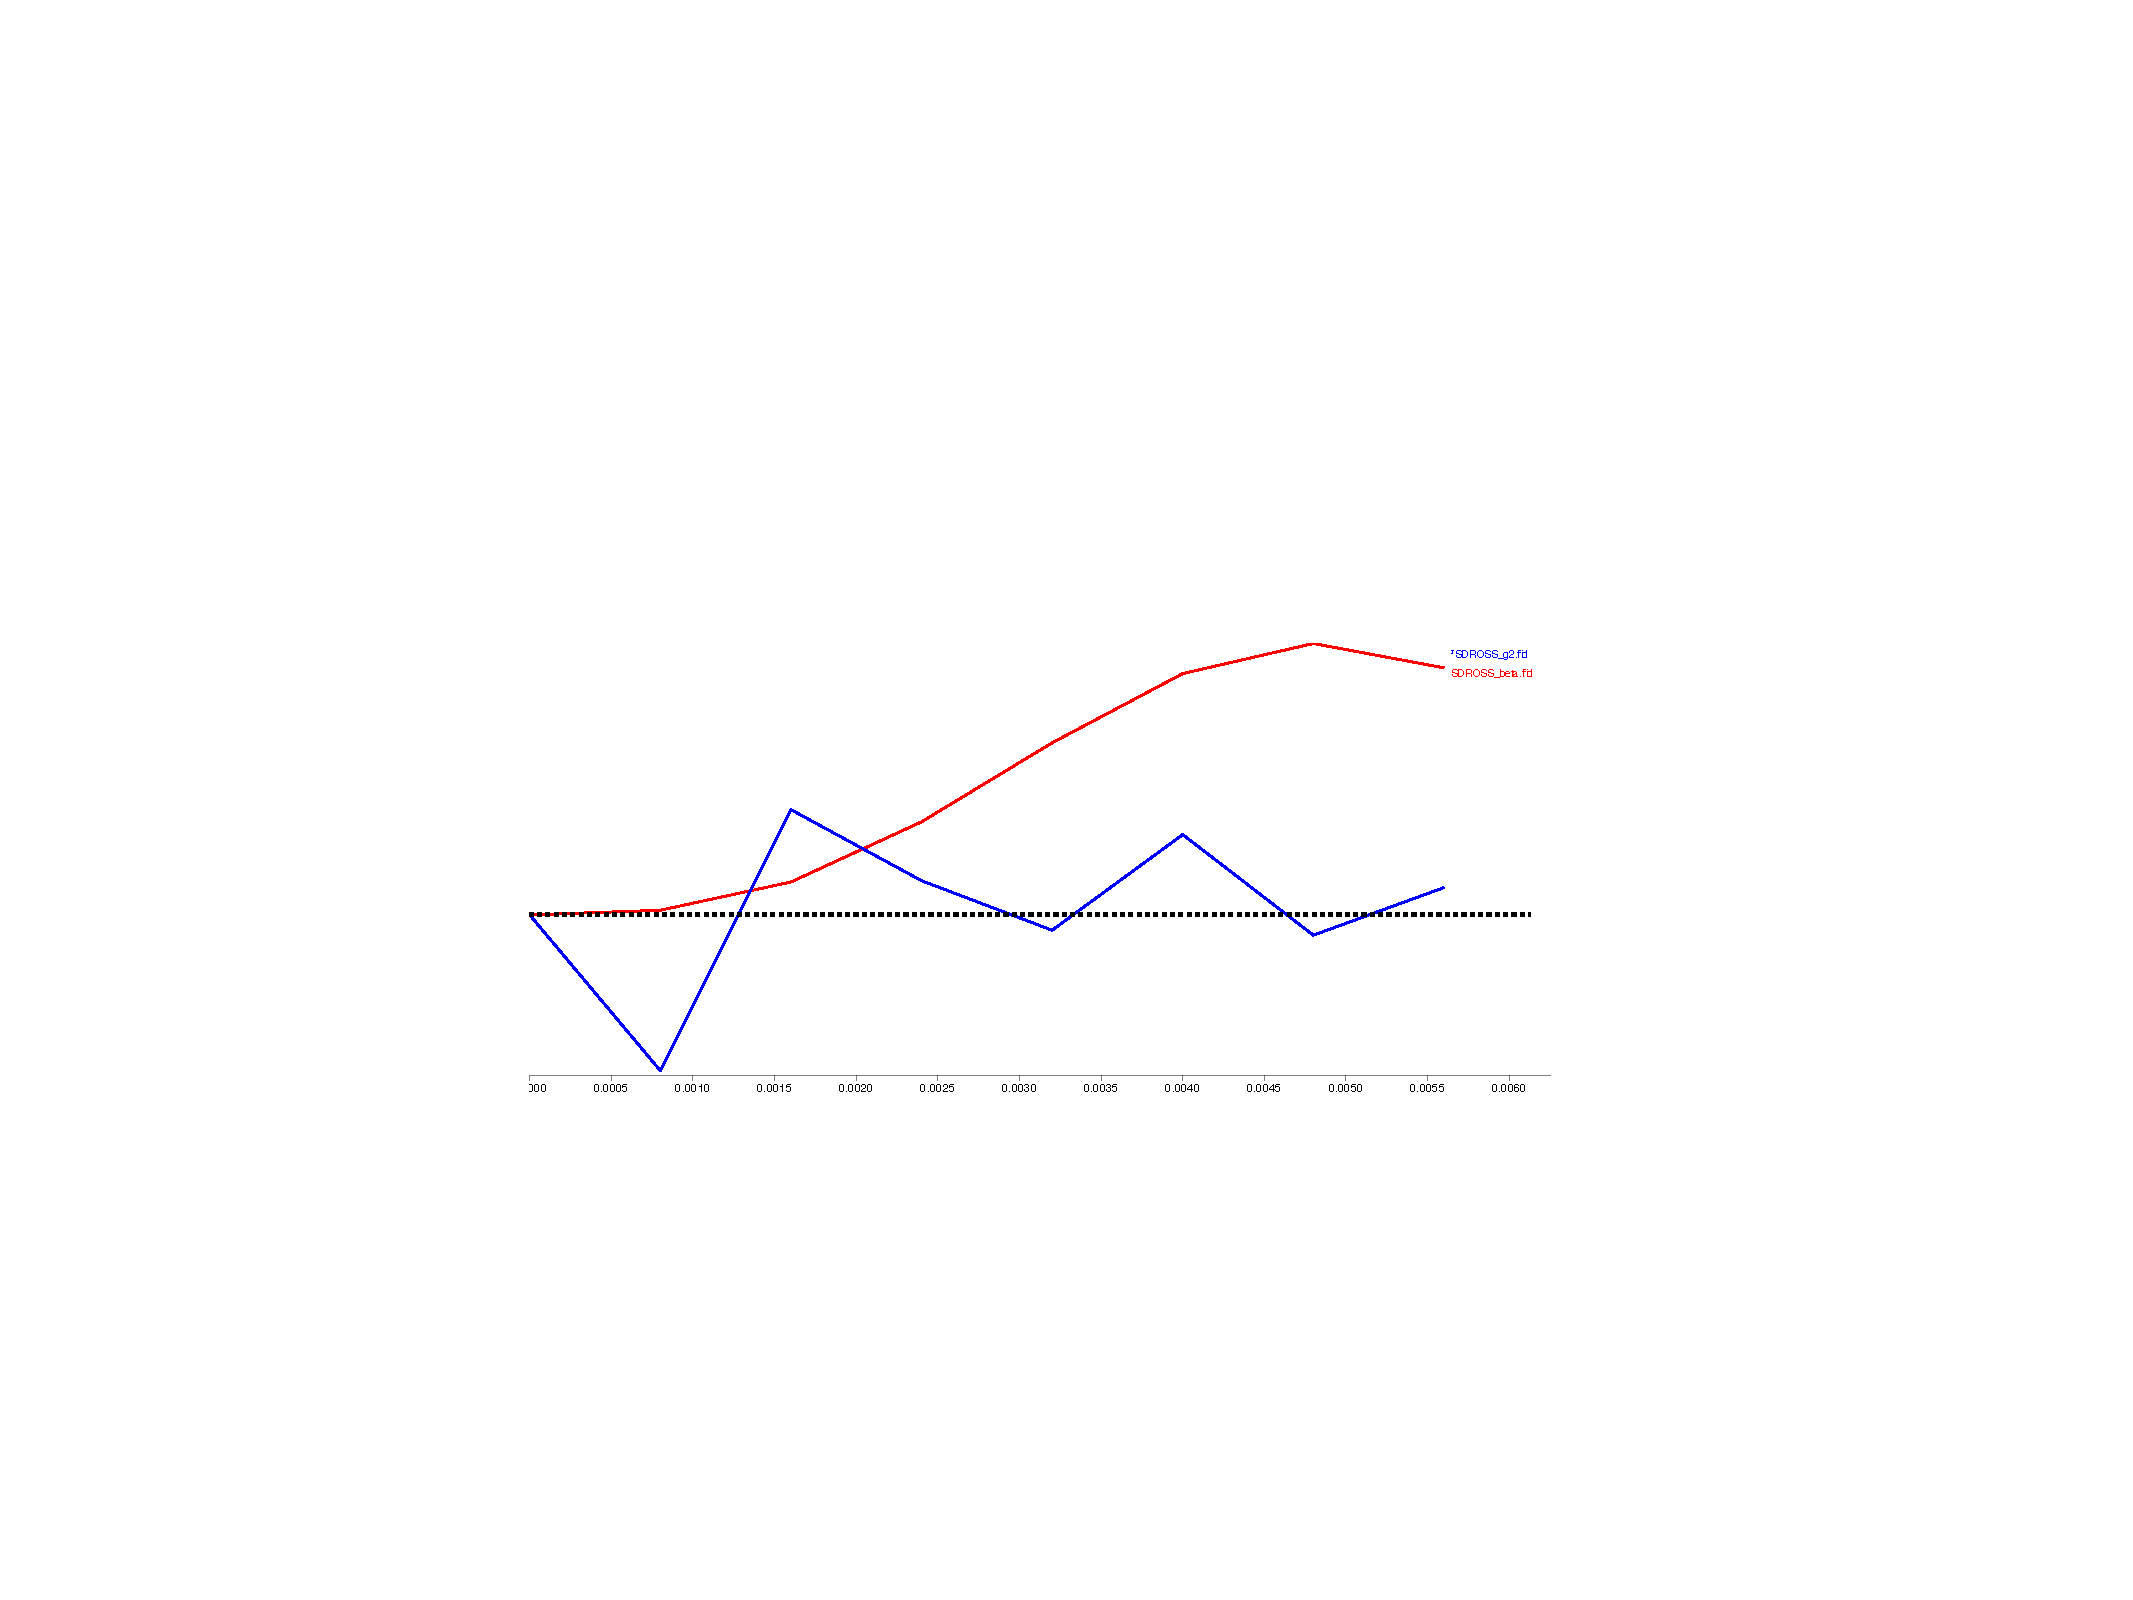
\includegraphics[width=0.8\textwidth]{../Figs/SIMPSON.pdf}
  \caption{\label{POPGsimpson}
    Simpson simulaton of S-DROSS curve of $\beta$-carbon of POPG.
  }
\end{figure}

\clearpage

\section{Changes of PG headroup order parameters upon addition of PC}

\begin{figure}[]
  \centering
  \includegraphics[width=8.0cm]{../Figs/HGorderparametersPGvsPC.eps}
  \caption{\label{HGorderparametersPGvsPC}
    Modulation of PG lipid headgroup order parameters with the increasing amount of PC in lipid bilayer
    from experiments \cite{borle85,macdonald87} and simulations with different force fields.
  }
\end{figure}

\clearpage

\section{Sodium binding to POPC simulations}

\begin{figure}[]
  \centering
  \includegraphics[width=8.0cm]{../Figs/NAdensPC.eps}
  \caption{\label{NAdensPC}
    Sodium (solid line) and choride ion density profiles along membrane normal
    from different simulations with PC lipids.
  }
  \todo{Discussion about differences to the NMRlipids II to be discussed once we have the details on ions models.}
\end{figure}



\bibliography{refs.bib}

\end{document}
